\documentclass[12pt, a4paper]{article}

% --- Packages ---
\usepackage[margin=2.5cm]{geometry}
\usepackage{setspace}
\usepackage{booktabs}
\usepackage{array}
\usepackage{longtable}
\usepackage{hyperref}
\usepackage[dvipsnames]{xcolor}
\usepackage{titlesec}
\usepackage{fancyhdr}
\usepackage{makecell}
\usepackage{graphicx}
\usepackage{amsmath}
\usepackage{amssymb}
\usepackage{enumitem}
\usepackage{parskip}
\usepackage[T1]{fontenc}
\usepackage{lmodern}
\usepackage[polish]{babel}
\usepackage[utf8]{inputenc}
\usepackage[backend=biber, style=ieee]{biblatex}
\usepackage{multirow}

\addbibresource{../SAP/references.bib}
\addto\captionspolish{
    \renewcommand{\figurename}{Rycina}
}
\definecolor{bayesPink}{HTML}{FF4D6D}
\definecolor{bayesPinkLight}{HTML}{FF8FA3}
\definecolor{bayesPurple}{HTML}{6A4C93}
\definecolor{bayesDark}{HTML}{2B2D42}
\newcommand{\todo}[1]{\textcolor{red}{\textbf{#1}}}
% --- Hyperref setup ---
\hypersetup{
    colorlinks = true,
    linkcolor  = bayesPurple,
    citecolor  = bayesPink,
    urlcolor   = bayesPinkLight
}

% --- Header/Footer ---
\pagestyle{fancy}
\fancyhf{}
\rhead{\textit{Raport z Analizy Statystycznej}}
\lhead{
\includegraphics[scale=0.2]{../SAP/graphics/logo-i-orzel.png}}
\rfoot{Strona \thepage}
\lfoot{\textit{}}

% --- Section formatting ---
\titleformat{\section}{\large\bfseries}{{\thesection}}{1em}{}[\titlerule]
\titleformat{\subsection}{\normalsize\bfseries}{{\thesubsection}}{1em}{}

% ============================================================
\begin{document}
% ============================================================

% --- Strona tytułowa ---
\begin{titlepage}
    \centering
    \vspace*{2cm}
    {\LARGE \textbf{Raport z Analizy Statystycznej} \par}
    \vspace{0.5cm}
    {\large Bayesowska analiza przeżycia róż: ocena skuteczności związków chemicznych w badaniu głównym\par}
    \vspace{2cm}
    \centering
    
\includegraphics[width=0.3\textwidth]{../SAP/graphics/UMB-logo.png}\par\vspace{2cm}

    \begin{tabular}{ll}
        \toprule
        \textbf{Wersja dokumentu}  & 1.0 \\
        \textbf{Data}              & \today \\
        \textbf{Autorzy}         & Julia Czyż, Urszula Skuńczyk, Paulina Włodarczyk\\
        \textbf{Afiliacja}         & Uniwersytet Medyczny w Białymstoku \\
                                   & Zakład Biostatystyki i Informatyki Medycznej \\
        \textbf{Odniesienie do SAP} & Plan Analizy Statystycznej, wersja 1.1 \\
        \bottomrule
    \end{tabular}

    \vspace{2cm}
    \vfill
\end{titlepage}

% --- Spis treści ---
\tableofcontents
\newpage

\onehalfspacing

% ============================================================
\section{Streszczenie}
% ============================================================
Niniejszy raport przedstawia wyniki bayesowskiej analizy przeżycia przeprowadzonej w celu identyfikacji związku chemicznego, który zapewni najdłuższy czas przeżycia kwiatu podczas transportu morskiego. Analizie z wykorzystaniem parametrycznego modelu Weibulla poddano 1920~jednostek eksperymentalnych (róż). Do dopasowania modelu wykorzystano pakiet \texttt{brms}~\cite{burkner2017brms}. W wyniku analizy stwierdzono, że związkiem chemicznym najefektywniej wydłużającym czas przeżycia kwiatu jest związek 6 -- \textit{Essence of Epiphaneia}, dla którego mediana a posteriori wyniosła: 20,5~dnia (95\%~CrI: [19,7;~21,3]).  
Prawdopodobieństwo przeżycia kwiatu przez typowy czas podróży (10~dni) wynosi dla tego związku 97,1\%, natomiast dla maksymalnego czasu podróży (22~dni)~--~38,7\%. Wszystkie łańcuchy MCMC osiągnęły zbieżność zgodnie z przyjętymi kryteriami.

% ============================================================
\section{Dane i przetwarzanie danych}
% ============================================================

\subsection{Źródło danych}

Dane do analizy głównej pochodziły z pliku \texttt{roses\_analysis2\_final.csv}. Schemat eksperymentu, definicje zmiennych oraz procedury przetwarzania danych zostały szczegółowo opisane w Planie Analizy Statystycznej (sekcje 2--3).

\subsection{Przetwarzanie danych}

Surowe dane o charakterze longitudinalnym przekształcono do postaci, w której dla każdej jednostki eksperymentalnej zachowano wyłącznie ostatni zarejestrowany pomiar czasu przeżycia (\texttt{time}). Ze względu na specyfikę implementacji modelu Weibulla w pakiecie \texttt{brms}, która uniemożliwia wprowadzenie obserwacji z czasem przeżycia równym 0, w przypadku takich jednostek za wartość zmiennej \texttt{time} przyjęto 0,5~dnia.

\subsection{Charakterystyka danych}

Zgodnie z założeniami w SAP (sekcja 2.5) dotyczącymi dostępności materiału eksperymentalnego, finalny zbiór danych obejmował pomiary dla 1920 jednostek eksperymentalnych, rozmieszczonych równomiernie w 48 komórkach eksperymentalnych (12 związków $\times$ 2 gatunki $\times$ 2 ogrody), po 40 kwiatów na każdą komórkę oraz 160 kwiatów dla każdego związku. Statystyki opisowe dla analizowanych związków zestawiono w Tabeli~\ref{tab:desc_stats}. Globalny odsetek obserwacji cenzurowanych wyniósł 1,9\% (36 jednostek), a najwyższy odsetek cenzurowania zaobserwowano dla związku 6, dla którego wyniósł on 12,5\%. 

\begin{table}[h!]
\centering
\footnotesize
\caption{Charakterystyka zbioru danych badania głównego według związku.}
\label{tab:desc_stats}
\begin{tabular}{clccccc}
\toprule
\textbf{ID} & \textbf{Nazwa związku} & \textbf{n} & \textbf{Liczba zdarzeń} & \textbf{Cenzur.} & \textbf{Cenzur. (\%)} & \thead{\textbf{Mediana KM} \\ \textbf{(dni)}} \\
\midrule
 1 & Distilled Water (kontrola)  & 160 & 160 &  0 &  0,0\% &  9,0 \\
\addlinespace
 4 & Concentrate of Caducues     & 160 & 160 &  0 &  0,0\% & 18,0 \\
 5 & Distillate of Discovery     & 160 & 157 &  3 &  1,9\% & 20,0 \\
 6 & Essence of Epiphaneia       & 160 & 140 & 20 & 12,5\% & 17,0 \\
 7 & Four in December            & 160 & 155 &  5 &  3,1\% & 12,5 \\
 8 & Granules of Geheref         & 160 & 159 &  1 &  0,6\% & 20,0 \\
 9 & Kar-Hamel Mooh              & 160 & 160 &  0 &  0,0\% & 15,0 \\
11 & Noospherol                  & 160 & 160 &  0 &  0,0\% & 20,0 \\
12 & Oil of John's Son           & 160 & 160 &  0 &  0,0\% & 19,5 \\
13 & Power of Perlimpinpin       & 160 & 160 &  0 &  0,0\% & 20,0 \\
14 & Spirit of Scienza           & 160 & 154 &  6 &  3,8\% & 16,5 \\
15 & Zest of Zen                 & 160 & 159 &  1 &  0,6\% & 17,0 \\
\addlinespace
\multicolumn{2}{l}{\textit{Łącznie}} & 1920 & 1884 &  36 &  1,9\% & -- \\
\bottomrule
\end{tabular}
\end{table}

% ============================================================
\section{Specyfikacja modelu}
% ============================================================
Pełna specyfikacja modelu określona została w SAP (sekcja~5). Poniżej zaś przedstawiono skrótowy opis modelu na potrzeby niniejszego raportu.

\subsection{Model Weibulla}

Czas przeżycia $T_i$ każdej $i$-tej róży modelowano parametrycznie przy użyciu rozkładu Weibulla:
\begin{equation}
    T_i \sim \mathrm{Weibull}(k,\,\lambda_i), \qquad
    S(t \mid k, \lambda_i) = \exp\!\left[-\!\left(\frac{t}{\lambda_i}\right)^{\!k}\right]
\end{equation}
Oczekiwany czas przeżycia modelowano na skali logarytmicznej:
\begin{equation}
    \log \mathbb{E}[T_i] = \beta_0 + \alpha_{c(i)} + \gamma_{s(i)} + \delta_{g(i)}
\end{equation}
gdzie $\beta_0$ to wyraz wolny, $\alpha_{c(i)}$ to efekt stały związku $c$ ($\alpha_1 = 0$ dla grupy kontrolnej), $\gamma_{s(i)}$ to efekt stały gatunku ($\gamma_1 = 0$ dla gatunku referencyjnego) oraz $\delta_{g(i)}$ to efekt stały ogrodu ($\delta_1 = 0$ dla ogrodu referencyjnego). Dla rozkładu Weibulla oczekiwany czas przeżycia wynosi $\mathbb{E}[T_i] = \lambda_i\cdot\Gamma(1+\frac{1}{k})$~\cite{stan_survival}, stąd parametr skali dla związku $c$ (przyjmując referencyjne poziomy gatunku i ogrodu) wyznaczany jest jako $\lambda_c = \exp(\beta_0 + \alpha_c)\,/\,\Gamma(1+\frac{1}{k})$~\cite{brms_families}.

Uśredniając po próbkach z rozkładu a~posteriori, otrzymujemy estymowaną medianę czasu przeżycia dla związku $c$. Górny indeks $(s)$ oznacza wartość parametru w $s$-tej iteracji MCMC (łącznie próbek a~posteriori $S = 4000$):
\begin{equation}
    \widehat{\mathrm{Me}}_c = \frac{1}{S}\sum_{s=1}^{S} \lambda_c^{(s)} \cdot (\ln 2)^{{\frac{1}{k}}^{(s)}}, \qquad
    \lambda_c^{(s)} = \frac{\exp\!\left(\beta_0^{(s)} + \alpha_c^{(s)}\right)}{\Gamma\!\left(1 + \frac{1}{k}^{(s)}\right)}
\end{equation}
Efekty $\alpha_c$ interpretowane są jako logarytm ilorazu średnich czasów przeżycia: $\exp(\alpha_c)$ jest czynnikiem, o~jaki zmienia się czas przeżycia kwiatu pod wpływem związku~$c$ względem grupy kontrolnej c$=1$.

\subsection{Rozkłady a priori}

Kalibracji rozkładów a priori dokonano na podstawie danych pilotażowych (szczegóły w SAP sekcja 5.3). W wyniku tego procesu otrzymano następujące informacyjne rozkłady a~priori dla parametrów modelu:

\begin{align}
    k       &\sim \mathrm{Gamma}(15{,}466;\;3{,}544) \\
    \beta_0 &\sim \mathcal{N}(2{,}918;\;0{,}362) \\
    \alpha_c,\;\gamma_s,\;\delta_g &\sim \mathcal{N}(0;\;0{,}24)
\end{align}

\subsection{Ustawienia MCMC}
Model dopasowano wykorzystując cztery niezależne łańcuchy Markowa. Zgodnie z przyjętymi w SAP założeniami (sekcja 7.1) dla każdego łańcucha wykonano 2000 iteracji, w tym 1000 iteracji przypadających na fazę rozgrzewania (ang. \textit{warmup}). W wyniku dopasowania uzyskano łącznie 4000 próbek z rozkładu a~posteriori. Jako backend próbkowania wykorzystano pakiet \texttt{cmdstanr}~\cite{cmdstanr}, który w porównaniu z domyślnym backendem \texttt{rstan} zapewnia szybszą kompilację modelu oraz dostęp do aktualnych optymalizacji algorytmu próbkowania.

% ============================================================
\section{Diagnostyka zbieżności łańcuchów MCMC}
% ============================================================

Zbieżność łańcuchów oceniono na podstawie statystyki $\hat{R}$ oraz efektywnej liczebności próby (Bulk-ESS i~Tail-ESS) zgodnie z~kryteriami~\cite{vehtari2019rhat}: $\hat{R} < 1{,}01$, Bulk-ESS~$> 400$, Tail-ESS~$> 400$ (szczegóły w SAP sekcja 7.2). Wyniki diagnostyki dla wszystkich parametrów modelu zestawiono w~Tabeli~\ref{tab:diagnostics}.

\begin{table}[h!]
\centering
\caption{Diagnostyka zbieżności łańcuchów MCMC.}
\label{tab:diagnostics}
\begin{tabular}{llccc}
\toprule
\textbf{Parametr} & \textbf{Opis} & \textbf{$\hat{R}$} & \textbf{Bulk-ESS} & \textbf{Tail-ESS} \\
\midrule
$k$             & Parametr kształtu           & 1,0012 & 2912 & 2679 \\
$\beta_0$       & Wyraz wolny (Intercept)      & 1,0018 & 1080 & 1791 \\
$\alpha_4$      & Concentrate of Caducues      & 1,0010 & 1396 & 2196 \\
$\alpha_5$      & Distillate of Discovery      & 1,0014 & 1306 & 2141 \\
$\alpha_6$      & Essence of Epiphaneia        & 1,0018 & 1409 & 2265 \\
$\alpha_7$      & Four in December             & 1,0012 & 1380 & 2123 \\
$\alpha_8$      & Granules of Geheref          & 1,0023 & 1372 & 2558 \\
$\alpha_9$      & Kar-Hamel Mooh               & 1,0012 & 1283 & 2101 \\
$\alpha_{11}$   & Noospherol                   & 1,0011 & 1375 & 1949 \\
$\alpha_{12}$   & Oil of John's Son            & 1,0013 & 1384 & 2137 \\
$\alpha_{13}$   & Power of Perlimpinpin        & 1,0019 & 1413 & 2321 \\
$\alpha_{14}$   & Spirit of Scienza            & 1,0014 & 1295 & 2188 \\
$\alpha_{15}$   & Zest of Zen                  & 1,0012 & 1385 & 2222 \\
$\gamma_s$      & Gatunek 2 (\textit{T.~hybrid}) & 1,0003 & 2940 & 2696 \\
$\delta_g$          & Ogród 2                  & 0,9999 & 3677 & 3029 \\
\bottomrule
\end{tabular}
\end{table}

Wszystkie parametry modelu spełniły przyjęte kryteria zbieżności, przy czym maksymalna wartość $\hat{R}$ wyniosła 1,0023 (dla $\alpha_8$), minimalna wartość Bulk-ESS wyniosła 1080 (dla $\beta_0$), a~minimalna wartość Tail-ESS wyniosła 1791 (dla $\beta_0$). Wyniki te świadczą o braku problemów ze zbieżnością łańcuchów, prawidłowym ich mieszaniu oraz efektywnym próbkowaniu z rozkładu a~posteriori.

\subsection{Wykresy przebiegu łańcuchów (trace plots)}

Rycina~\ref{fig:trace} przedstawia przebiegi czterech łańcuchów Markowa dla wybranych parametrów modelu: parametru kształtu~$k$, wyrazu wolnego~$\beta_0$, efektu najlepszego związku~$\alpha_6$ oraz efektu związku o~najmniejszym wpływie~$\alpha_9$. Łańcuchy prawidłowo oscylują wokół stałej wartości (,,włochata gąsienica''), mieszając się ze sobą.

\begin{figure}[h!]
    \centering
    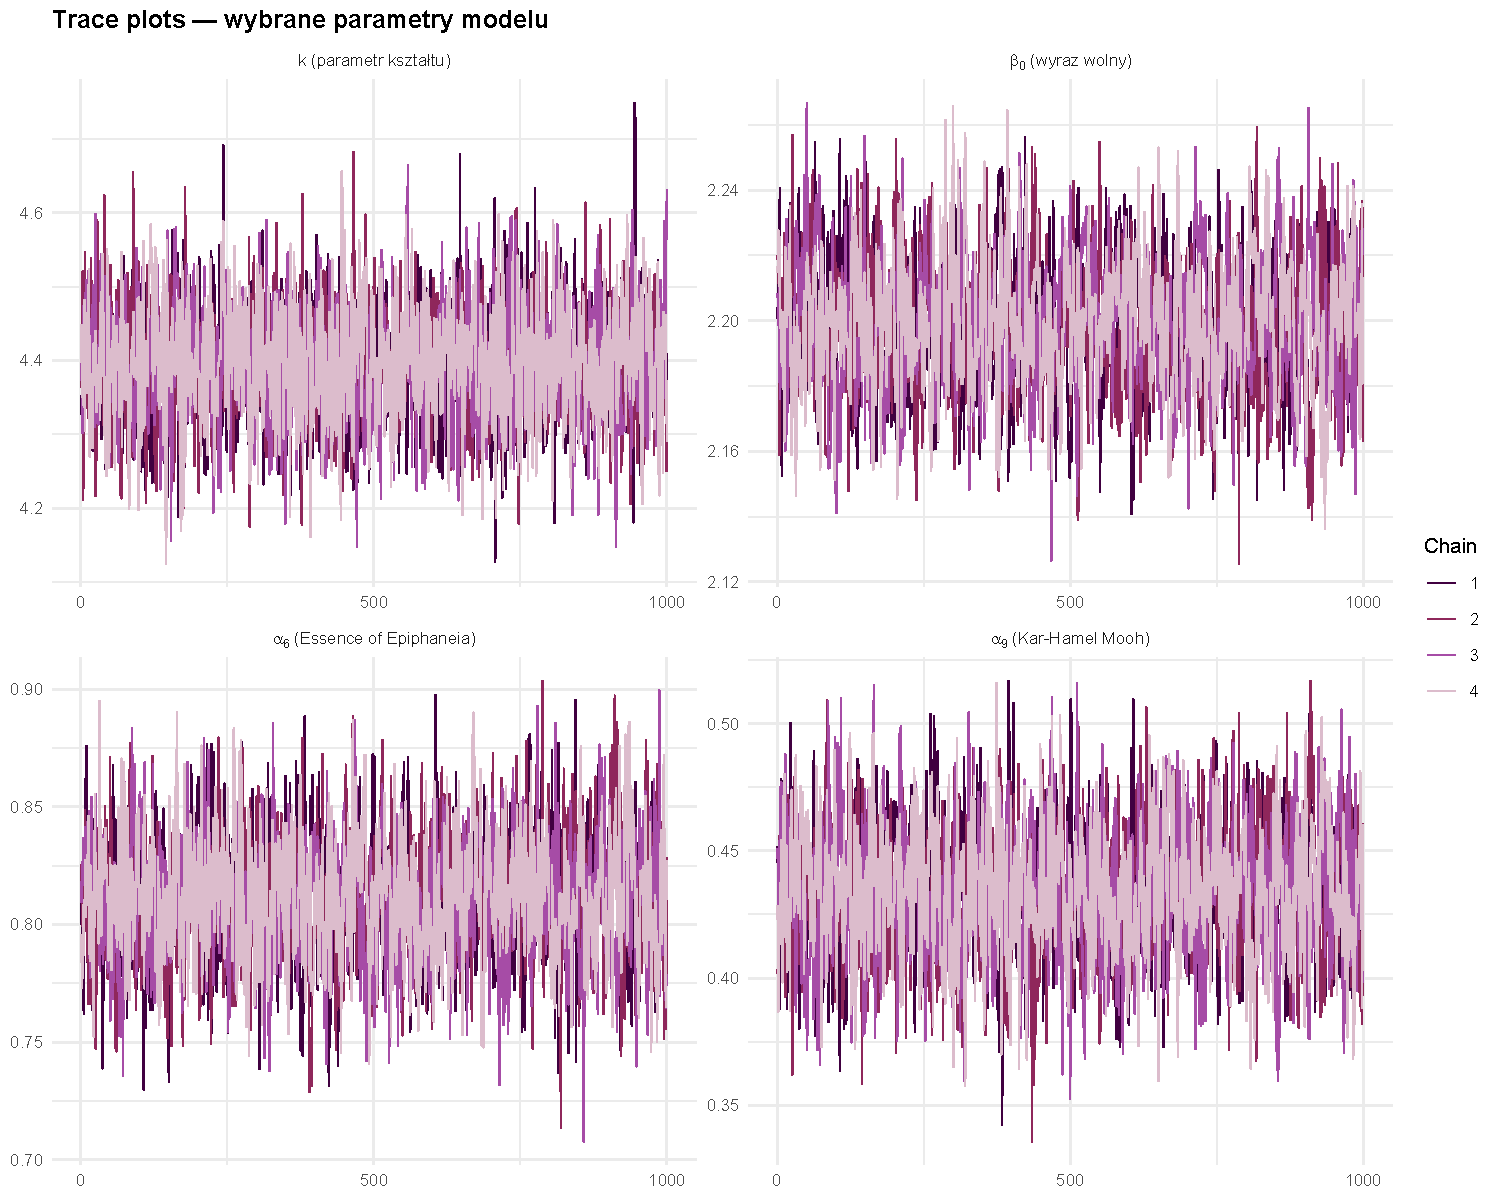
\includegraphics[width=1.0\textwidth]{../plots/trace_plots.pdf}
    \caption{Wykresy przebiegu łańcuchów dla wybranych parametrów modelu ($k$, $\beta_0$, $\alpha_6$, $\alpha_9$).}
    \label{fig:trace}
\end{figure}

\subsection{Autokorelacja wewnątrz łańcuchów}

Rycina~\ref{fig:acf} przedstawia wykresy autokorelacji kolejnych próbek dla tych samych parametrów przy opóźnieniach (lag) od~1 do~20. Szybki zanik autokorelacji potwierdza wysoką efektywność próbkowania i tłumaczy wysokie wartości ESS uzyskane dla wszystkich parametrów. 

\begin{figure}[h!]
    \centering
    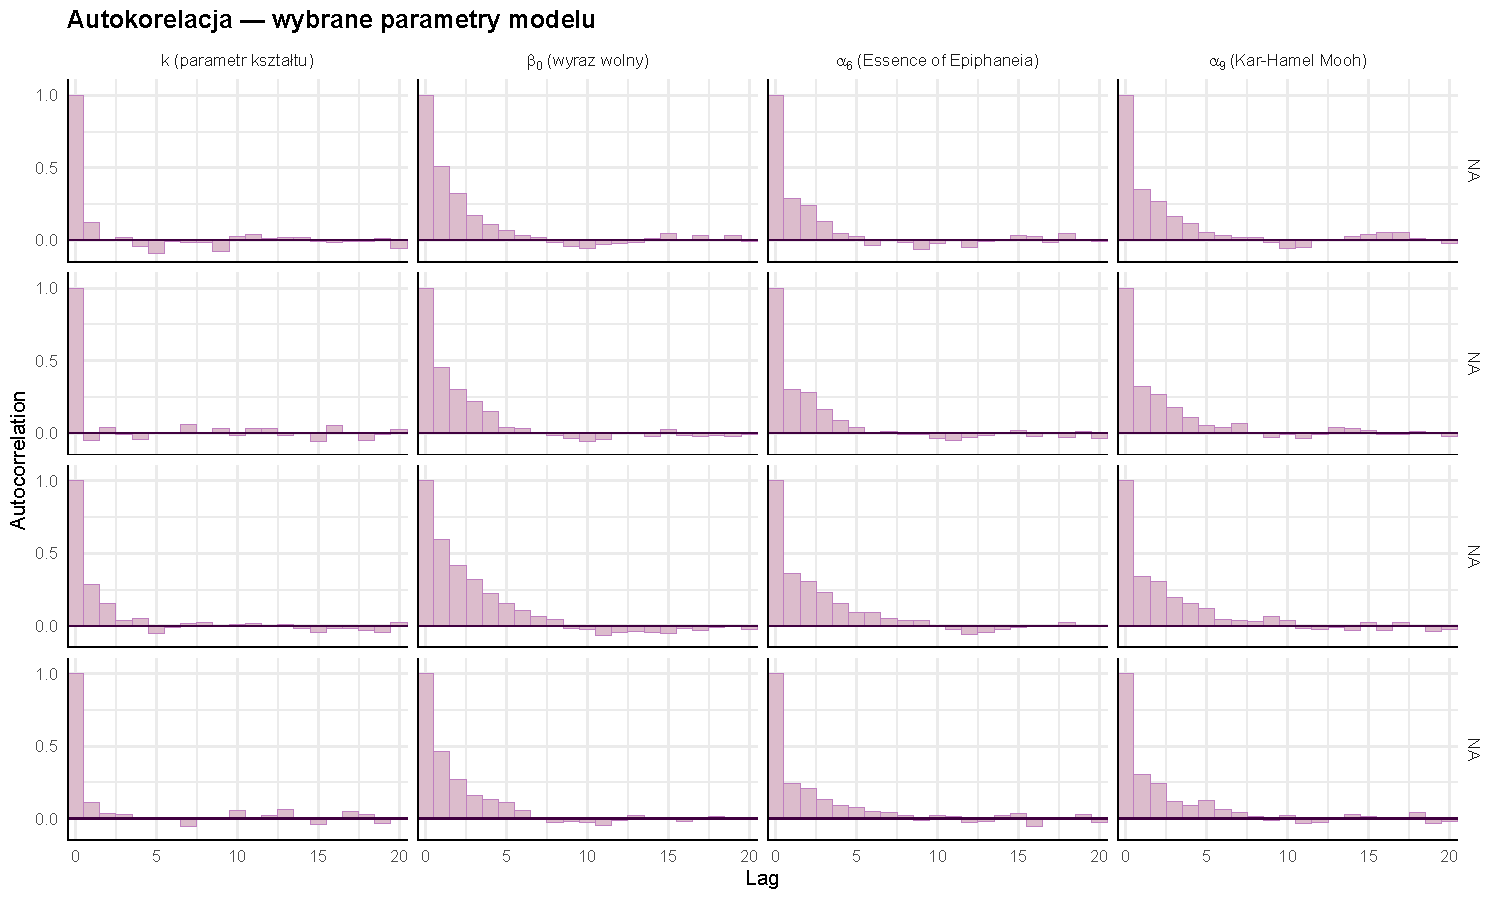
\includegraphics[width=1.0\textwidth]{../plots/acf_plots.pdf}
    \caption{Wykresy autokorelacji (ACF) dla wybranych parametrów modelu.}
    \label{fig:acf}
\end{figure}

\subsection{Wykresy rang}

Rycina~\ref{fig:rank} przedstawia wykresy rozkładu rang (ang.~\textit{rank overlay plots})~\cite{vehtari2019rhat} dla wybranych parametrów. Rangi próbek z poszczególnych łańcuchów rozkładają się równomiernie wokół wartości oczekiwanej (~50), bez wyraźnej dominacji któregokolwiek łańcucha. Świadczy to o dobrej zbieżności próbkowania i właściwym mieszaniu łańcuchów dla wszystkich analizowanych parametrów.
\begin{figure}[h!]
    \centering
    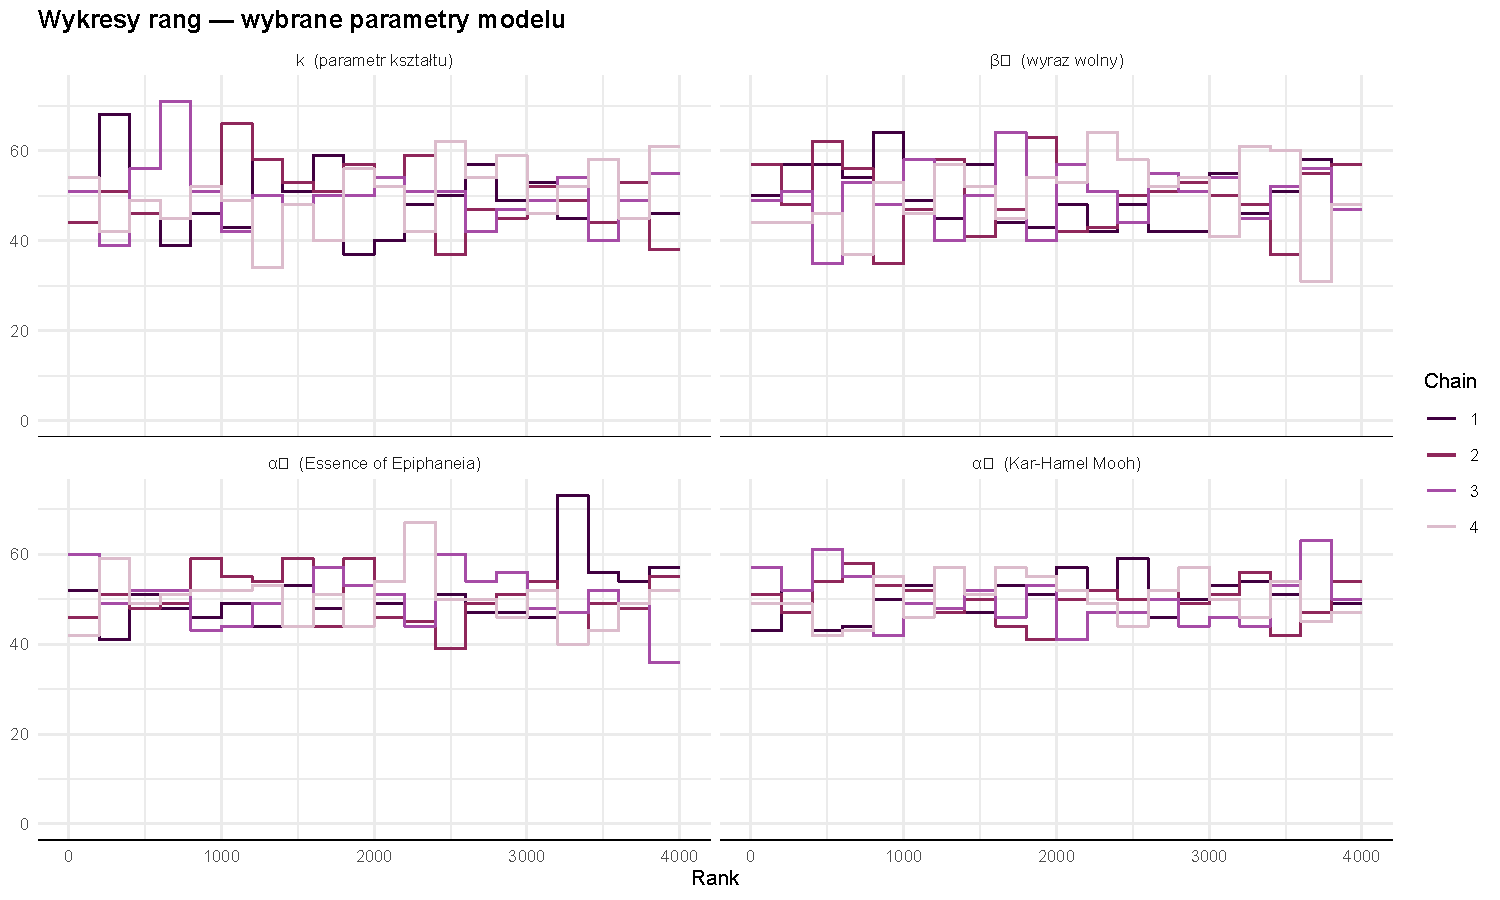
\includegraphics[width=1.0\textwidth]{../plots/rank_plots.pdf}
    \caption{Wykresy rang dla wybranych parametrów modelu. }
    \label{fig:rank}
\end{figure}
\clearpage
\newpage
% ============================================================
\section{Wyniki analizy głównej}
% ============================================================

\subsection{Ocena dopasowania modelu -- posterior predictive check}

W celu oceny adekwatności dopasowania modelu Weibulla do danych przeprowadzono posterior predictive check. Dla każdego z analizowanych związków zestawiono bayesowskie krzywe przeżycia a~posteriori z~empirycznym estymatorem Kaplana-Meiera wyznaczonym z~danych. Graficzne podsumowanie porównania przedstawia Rycina~\ref{fig:ppc}.

\begin{figure}[h!]
    \centering
    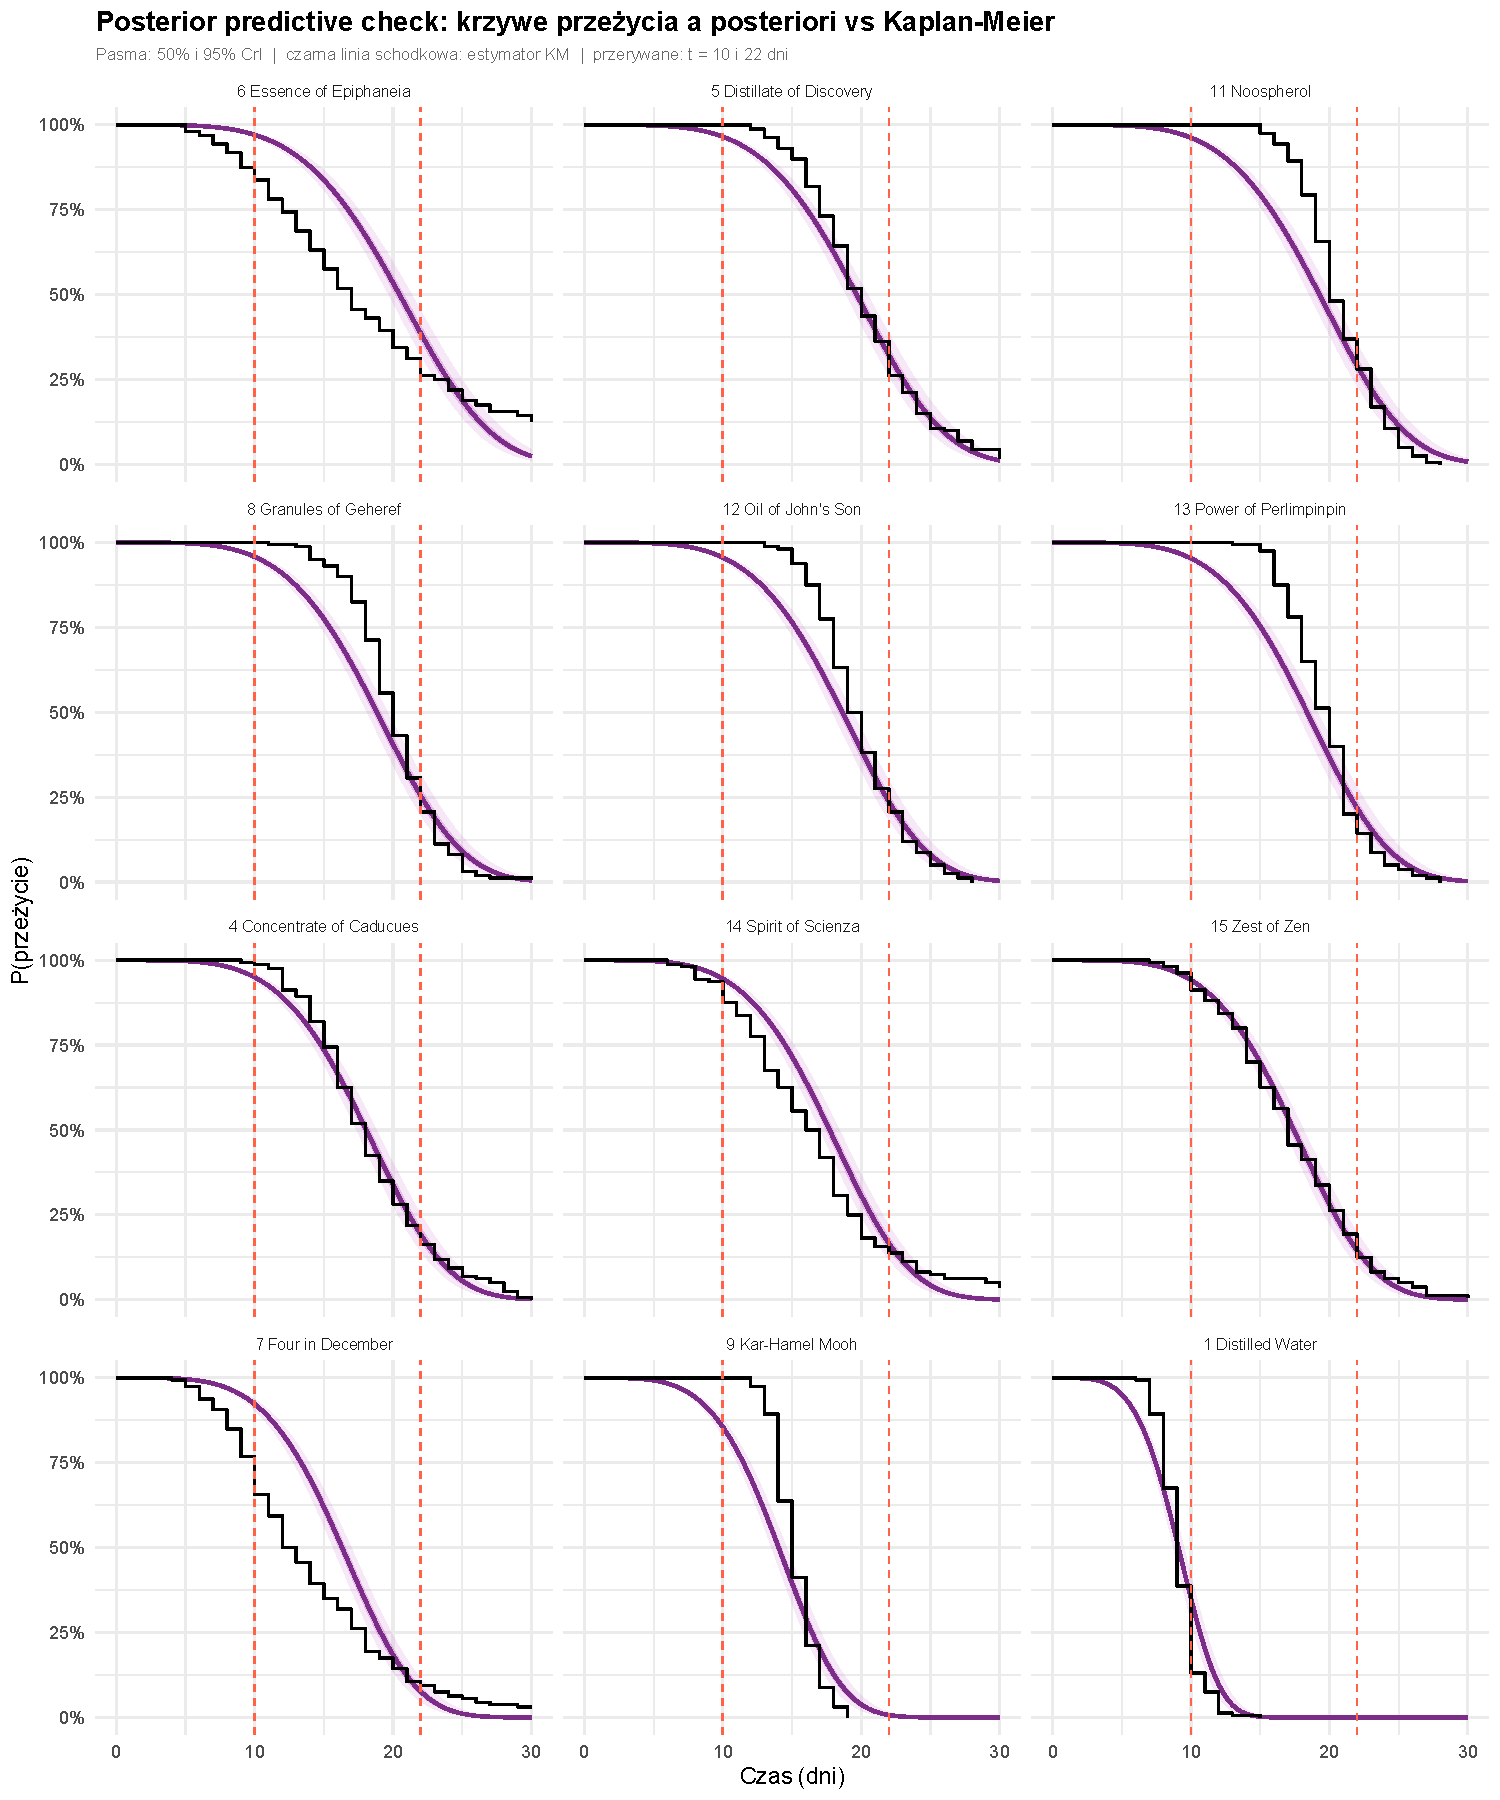
\includegraphics[width=1.0\textwidth, height=14cm]{../plots/ppc_km.pdf}
    \caption{Posterior predictive check: bayesowskie krzywe przeżycia a posteriori (fioletowe pasma) nałożone na estymator Kaplana-Meiera (czarna linia schodkowa). Uporządkowane według otrzymanego rankingu związków.}
    \label{fig:ppc}
\end{figure}

W przypadku związków 4 (\textit{Concentrate of Caducues}) oraz~ 15 (\textit{Zest of Zen}) zaobserwowano niemalże idealną zgodność estymatora KM z~krzywą przeżycia a~posteriori na całej długości przedziału. 

Dla związków~1 (\textit{Distilled Water}), 5 (\textit{Distillate of Discovery}) oraz~14 (\textit{Spirit of Scienza}) odnotowano niewielkie, lokalne odchylenia estymatora KM poza granice 95\%~CrI, ograniczone do krótkiego przedziału czasowego i~o~małej amplitudzie, co uznano za dopasowanie akceptowalne.

Dla związków~11 (\textit{Noospherol}), 8 (\textit{Granules of Geheref}), 12 (\textit{Oil of John's Son}), 13 (\textit{Power of Perlimpinpin}) oraz~9 (\textit{Kar-Hamel Mooh}) estymator KM przebiega wyraźnie powyżej krzywej przeżycia a~posteriori w~środkowej fazie obserwacji, co może 
sugerować systematyczną tendencję modelu Weibulla do niedoszacowania przeżycia w~tym przedziale czasowym dla wspomnianych grup.

Odwrotną tendencję zaobserwowano dla związków~6 (\textit{Essence of Epiphaneia}) oraz~7 (\textit{Four in December}), dla których estymator 
KM przebiega wyraźnie poniżej krzywej przeżycia a~posteriori na przedziale 5--20~dni, co wskazuje na zawyżenie czasu przeżycia przez model Weibulla w~tych grupach.

Największe zastrzeżenie z~punktu widzenia głównego celu analizy stanowi przeszacowanie czasu przeżycia przez model dla związków~6 (\textit{Essence of Epiphaneia}) oraz~7 (\textit{Four in December}), co zostało szerzej omówione w sekcji poświęconej dyskusji.

\subsection{Rozkłady a posteriori parametrów modelu}

W~Tabeli~\ref{tab:posterior_summary} przedstawiono średnie a~posteriori oraz 95\%~przedziały wiarygodności dla wszystkich parametrów modelu.

\begin{table}[h!]
\centering
\caption{Podsumowanie rozkładów a posteriori parametrów modelu.}
\label{tab:posterior_summary}
\begin{tabular}{llcc}
\toprule
\textbf{Parametr} & \textbf{Opis} & \textbf{Średnia a posteriori} & \textbf{95\% CrI} \\
\midrule
$k$                  & Parametr kształtu             & 4,395  & [4,243;\; 4,547] \\
$\beta_0$            & Wyraz wolny                   & 2,199  & [2,159;\; 2,239] \\
\addlinespace
$\alpha_4$           & Concentrate of Caducues       & 0,686  & [0,633;\; 0,737] \\
$\alpha_5$           & Distillate of Discovery       & 0,771  & [0,719;\; 0,822] \\
$\alpha_6$           & Essence of Epiphaneia         & 0,811  & [0,760;\; 0,866] \\
$\alpha_7$           & Four in December              & 0,584  & [0,532;\; 0,638] \\
$\alpha_8$           & Granules of Geheref           & 0,728  & [0,676;\; 0,781] \\
$\alpha_9$           & Kar-Hamel Mooh                & 0,434  & [0,382;\; 0,484] \\
$\alpha_{11}$        & Noospherol                    & 0,752  & [0,698;\; 0,805] \\
$\alpha_{12}$        & Oil of John's Son             & 0,717  & [0,665;\; 0,768] \\
$\alpha_{13}$        & Power of Perlimpinpin         & 0,704  & [0,650;\; 0,756] \\
$\alpha_{14}$        & Spirit of Scienza             & 0,666  & [0,614;\; 0,716] \\
$\alpha_{15}$        & Zest of Zen                   & 0,650  & [0,598;\; 0,702] \\
\addlinespace
$\gamma_s$           & Gatunek 2 (\textit{T.~hybrid}) & 0,026 & [0,005;\; 0,048] \\
$\delta_g$           & Ogród 2                       & 0,004  & [-0,017;\; 0,025] \\
\bottomrule
\end{tabular}
\end{table}

Estymowany parametr kształtu $k = 4{,}395$ (95\%~CrI: [4,243;~4,547]) potwierdza narastający charakter hazardu ($k > 1$), zgodny z~biologicznym procesem pogarszania się kondycji kwiatów w~czasie. Wszystkie efekty związków $\alpha_c > 0$ oraz żaden z przedziałów wiarygodności nie zawiera 0, oznacza to, że każda z badanych substancji istotnie wydłuża czas przeżycia kwiatów w porównaniu z grupą kontrolną. W przypadku najlepszego związku \textit{acceleration factor} $\exp(\alpha_c)$ wynosi $\exp(0{,}811) \approx 2{,}25$, co oznacza, że owy związek wydłuża oczekiwany czas przeżycia 2,25-krotnie względem kontroli. Efekt gatunku ($\gamma_s = 0{,}026$) jest niewielki, lecz istotny, natomiast efekt ogrodu ($\delta_g = 0{,}004$; CrI zawiera zero) jest pomijalny.

\subsection{Pierwszorzędowy punkt końcowy: ranking związków}\label{subsec:ranking}

Pierwszorzędowym punktem końcowym był ranking związków według mediany czasu przeżycia wyznaczonej z~rozkładu a~posteriori. Wyniki przedstawiono w~Tabeli~\ref{tab:compound_ranking} oraz na Rycinie~\ref{fig:compound_ranking}.

\begin{table}[h!]
\centering
\caption{Ranking związków według mediany czasu przeżycia a posteriori wraz z prawdopodobieństwami przeżycia dla typowego ($t = 10$~dni) i~maksymalnego ($t = 22$~dni) czasu podróży.}
\label{tab:compound_ranking}
\begin{tabular}{clp{4.2cm}cccc}
\toprule
\textbf{Ranga} & \textbf{ID} & \textbf{Nazwa związku} & \textbf{Mediana (dni)} & \textbf{95\% CrI (dni)} & $\hat{S}(10)$ & $\hat{S}(22)$ \\
\midrule
 1 &  6 & Essence of Epiphaneia     & 20,5 & [19,7;\; 21,3] & 97,1\% & 38,7\% \\
 2 &  5 & Distillate of Discovery   & 19,7 & [18,9;\; 20,4] & 96,5\% & 32,2\% \\
 3 & 11 & Noospherol                & 19,3 & [18,6;\; 20,1] & 96,2\% & 29,1\% \\
 4 &  8 & Granules of Geheref       & 18,8 & [18,2;\; 19,6] & 95,8\% & 25,5\% \\
 5 & 12 & Oil of John's Son         & 18,6 & [18,0;\; 19,4] & 95,6\% & 23,7\% \\
 6 & 13 & Power of Perlimpinpin     & 18,4 & [17,7;\; 19,1] & 95,3\% & 21,9\% \\
 7 &  4 & Concentrate of Caducues   & 18,1 & [17,4;\; 18,8] & 95,0\% & 19,4\% \\
 8 & 14 & Spirit of Scienza         & 17,7 & [17,0;\; 18,4] & 94,5\% & 16,7\% \\
 9 & 15 & Zest of Zen               & 17,4 & [16,8;\; 18,1] & 94,1\% & 14,7\% \\
10 &  7 & Four in December          & 16,3 & [15,7;\; 17,0] & 92,2\% &  7,7\% \\
11 &  9 & Kar-Hamel Mooh            & 14,0 & [13,5;\; 14,6] & 85,5\% &  0,7\% \\
\addlinespace
-- &  1 & Distilled Water (kontrola) & 9,1 & [8,74;\; 9,48] & 35,0\% & $< 0{,}1$\% \\
\bottomrule
\end{tabular}
\end{table}

\begin{figure}[h!]
    \centering
    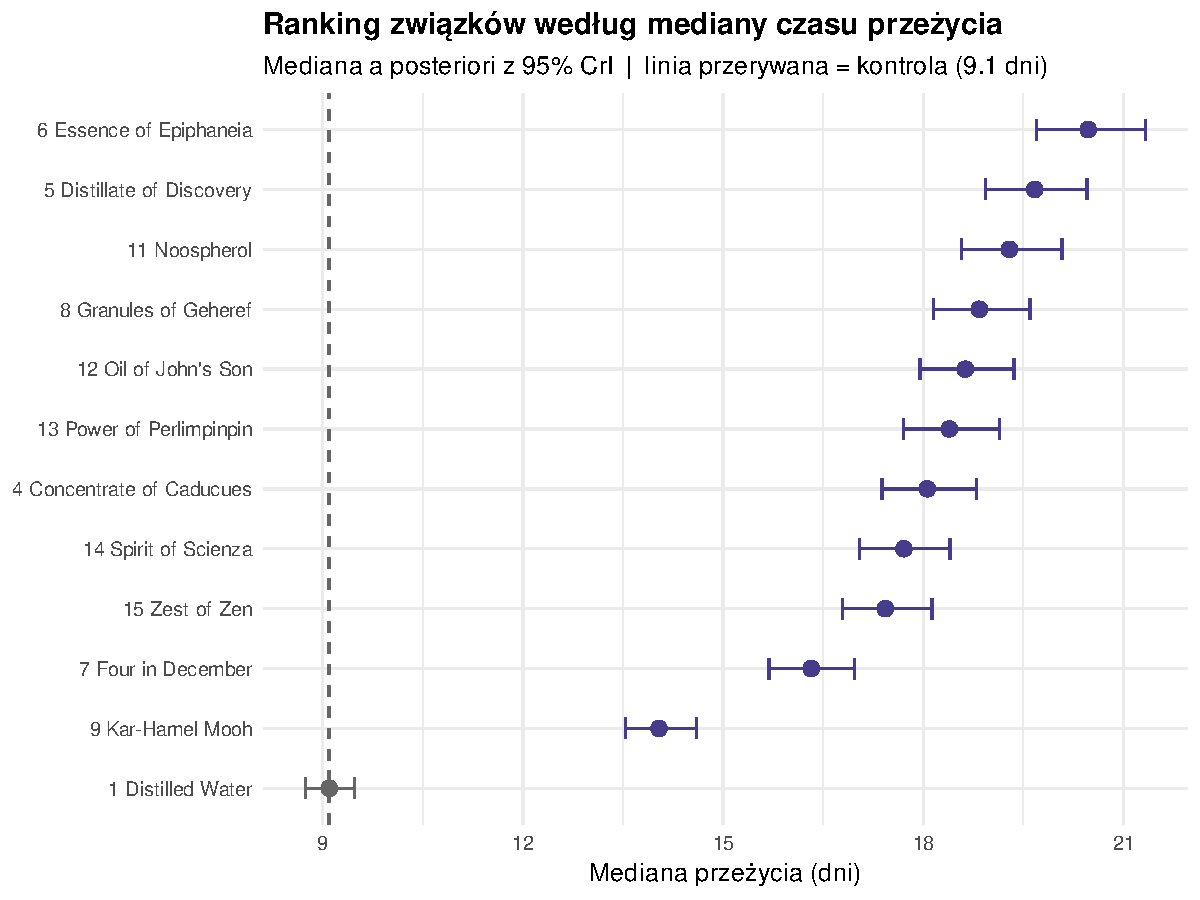
\includegraphics[width=0.85\textwidth]{../plots/compound_ranking.pdf}
    \caption{Ranking związków według mediany czasu przeżycia a posteriori. Punkty: mediana; odcinki poziome: 95\% CrI; linia przerywana: mediana grupy kontrolnej (9,1~dnia).}
    \label{fig:compound_ranking}
\end{figure}

\par W~rankingu pierwsze miejsce zajął związek~6 (\textit{Essence of 
Epiphaneia}) z~estymowaną medianą czasu przeżycia 20,5~dnia 
(95\%~CrI: [19,7;~21,3]). Przedział wiarygodności związku~6 częściowo 
zachodzi na przedział związku~5 (\textit{Distillate of Discovery}, 
mediana 19,7~dnia, 95\%~CrI: [18,9;~20,4]), który zajął drugie miejsce, 
co wskazuje na pewną niepewność w~jednoznacznym rozstrzygnięciu przewagi 
jednego z~nich nad drugim. Kolejność związków na pozycjach 3--7 (mediana 
w~zakresie 18,1--19,3~dnia) jest obarczona jeszcze większą niepewnością 
ze względu na szeroko nakładające się przedziały wiarygodności. Wszystkie badane substancje wykazały istotnie dłuższy czas przeżycia 
w~porównaniu z~grupą kontrolną (\textit{Distilled Water}, mediana 
9,1~dnia).

\subsection{Drugorzędowe punkty końcowe: prawdopodobieństwa przeżycia}

\subsubsection{Przeżycie przez typowy czas podróży ($t = 10$~dni)}

Dla podróży trwającej typowo 10 dni wszystkie badane substancje zapewniają stosunkowo wysokie prawdopodobieństwo przeżycia kwiatu (Tabela~\ref{tab:compound_ranking}). Dla związku 6 sklasyfikowanego na pierwszym miejscu w rankingu prawdopodobieństwo to wyniosło aż $97{,}1\%$. Nawet dla najsłabszego spośród ocenianych związków -- 9 (\textit{Kar-Hamel Mooh}) wartość ta wyniosła $85{,}5\%$. W~porównaniu z~grupą kontrolną ($\hat{S}(10) = 35{,}0\%$) zastosowanie któregokolwiek ze związków zwiększa prawdopodobieństwo przeżycia 
kwiatu o~co najmniej 50,5~punktu procentowego.

\subsubsection{Przeżycie przez maksymalny czas podróży ($t = 22$~dni)}

Dla maksymalnego spodziewanego czasu podróży wynoszącego 22~dni 
zróżnicowanie między związkami jest zdecydowanie większe. Żaden 
z~badanych związków nie osiąga progu 50\% prawdopodobieństwa przeżycia; 
najwyższą wartość odnotowano dla związku~6 ($\hat{S}(22) = 38{,}7\%$). 
Dla związku~9 (\textit{Kar-Hamel Mooh}) oraz grupy kontrolnej 
prawdopodobieństwo przeżycia kwiatu jest bliskie zeru (odpowiednio 
0,7\% i~$<$0,1\%). Wyniki te wskazują, że w~najbardziej pesymistycznym 
scenariuszu czasowym szanse na utrzymanie kwiatu w~dobrej kondycji 
pozostają niskie nawet przy zastosowaniu najskuteczniejszego preparatu.

% ============================================================
\section{Analiza wrażliwości}
% ============================================================

Zgodnie z~SAP (sekcja~6) przeprowadzono analizę wrażliwości polegającą na dopasowaniu modelu z~analogicznymi słabo informacyjnymi rozkładami a~priori:
\begin{align}
    k &\sim \mathrm{Gamma}(2;\;0{,}5) \\
    \beta_0 &\sim \mathcal{N}(0;\;1) \\
    \alpha_c,\;\gamma_s,\;\delta_g &\sim \mathcal{N}(0;\;1)
\end{align}

Porównanie median a~posteriori efektów związków w~kolejności rankingowej 
między modelem głównym a~modelem dopasowanym z~rozkładami słabo 
informacyjnymi przedstawiono w~Tabeli~\ref{tab:sensitivity}. Zachowana 
jest pełna zgodność rankingu, a~wyniki są niemalże identyczne dla obu 
modeli. Jedyna zauważalna różnica dotyczy grupy kontrolnej (9,1 oraz 
8,7~dnia), co wynika z~wpływu rozkładu a~priori parametru $\beta_0$ 
skalibrowanego na danych pilotażowych. Otrzymane wyniki analizy 
wrażliwości potwierdzają, że przyjęte rozkłady a~priori dla modelu 
głównego nie zdominowały finalnych wniosków z~analizy.

\begin{table}[h!]
\centering
\footnotesize
\caption{Porównanie median czasu przeżycia: model główny vs.~model wrażliwości.}
\label{tab:sensitivity}
\begin{tabular}{clcc}
\toprule
\textbf{ID} & \textbf{Nazwa związku} & \textbf{Mediana -- model główny (dni)} & \textbf{Mediana -- model wrażliwości (dni)} \\
\midrule
 6 & Essence of Epiphaneia     & 20,5 & 20,6 \\
 5 & Distillate of Discovery   & 19,7 & 19,8 \\
11 & Noospherol                & 19,3 & 19,4 \\
 8 & Granules of Geheref       & 18,8 & 18,9 \\
12 & Oil of John's Son         & 18,6 & 18,7 \\
13 & Power of Perlimpinpin     & 18,4 & 18,5 \\
 4 & Concentrate of Caducues   & 18,1 & 18,1 \\
14 & Spirit of Scienza         & 17,7 & 17,8 \\
15 & Zest of Zen               & 17,4 & 17,5 \\
 7 & Four in December          & 16,3 & 16,4 \\
 9 & Kar-Hamel Mooh            & 14,0 & 14,1 \\
 1 & Distilled Water (kontrola) & 9,1 & 8,7 \\
\bottomrule
\end{tabular}
\end{table}

% ============================================================
\section{Dyskusja}
% ============================================================

\subsection{Zasadność wyboru rozkładu Weibulla}

Zasadność wyboru modelu Weibulla potwierdzona została w analizie głównej, w której estymowana wartość parametru kształtu wyniosła $k = 4{,}395$ (95\%~CrI: [4,243;~4,547]), która dostarcza informacji na temat narastającego w czasie ryzyka obumarcia kwiatu, co jest biologicznie wiarygodne dla omawianego procesu starzenia się ciętych kwiatów.

Posterior predictive check (Rycina~\ref{fig:ppc}) wykazał zróżnicowanie w dokładności dopasowania modelu do danych. Dla związków 4 oraz 15 zaobserwowano niemal idealną zgodność między krzywą Kaplana-Meiera a krzywą przeżycia a~posteriori. Dla części związków (8, 9, 11, 12, 13) model Weibulla konsekwentnie zaniżał prawdopodobieństwo przeżycia w~środkowej fazie obserwacji, podczas gdy dla związków~6 i~7 przewidywał prawdopodobieństwo przeżycia wyższe niż obserwowane empirycznie. Szczególną uwagę należy zwrócić na związek 6 (\textit{Essence of Epiphaneia}), dla którego różnica między medianą KM (17 dni) a medianą a~posteriori (20,5 dnia) wyniosła aż 3,5 dnia. Rozbieżność ta wynikać może po części z najwyższego w badaniu odsetka obserwacji cenzurowanych (12,5\%), który zmniejsza ilość informacji dostępnej do estymacji metodą Kaplana–Meiera i zwiększa niepewność wyznaczenia mediany przeżycia. Model bayesowski, wykorzystując dodatkowo informację zawartą w~rozkładzie a~priori oraz założenia parametryczne rozkładu Weibulla, dał wyższe oszacowanie mediany, które może lepiej odzwierciedlać rzeczywisty czas przeżycia w~tej grupie.

Warto zauważyć, że obserwowany dla części związków wzorzec krzywej KM -- długi początkowy okres niewielkiego ryzyka, po którym następuje gwałtowny wzrost umieralności (np.~związki~7, 11) -- może wskazywać na hazard o~przebiegu bardziej złożonym niż zakładany przez rozkład Weibulla, który z~definicji jest monotoniczny (stale rosnący lub stale malejący). Rozbieżności zaobserwowane w~posterior predictive check dla części związków mogą być więc po części konsekwencją ograniczenia przyjętej specyfikacji. W~przyszłych analizach warto byłoby rozważyć alternatywne rozkłady dopuszczające zmienny w~czasie (niemonotoniczny) kształt funkcji hazardu, takie jak rozkład log-normalny lub log-logistyczny, które mogłyby lepiej odzwierciedlać opisany wzorzec i~potencjalnie poprawić dokładność dopasowania modelu do danych.
\subsection{Wpływ rozkładów a priori}

Rozkłady a~priori parametrów modelu skalibrowano na podstawie danych pilotażowych. Przy liczebności grup wynoszącej $n = 160$ obserwacji wkład rozkładów a~priori w rozkład a~posteriori był relatywnie niewielki, ponieważ głównym źródłem informacji w procesie estymacji były dane obserwacyjne. Przeprowadzona analiza wrażliwości wykazała, że zastąpienie rozkładów informacyjnych słabo informacyjnymi skutkuje różnicami median nie przekraczającymi 0,1~dnia dla wszystkich związków, z wyjątkiem grupy kontrolnej (9,1 vs.~8,7~dnia), co wynika z~wpływu rozkładu a~priori wyrazu wolnego $\beta_0$ na estymację bazowego czasu przeżycia. Kolejność rankingu ze względu na medianę przeżycia została w pełni zachowana.

\subsection{Ograniczenia analizy}

Należy wskazać kilka ograniczeń niniejszej analizy. Po pierwsze, badanie obejmowało wyłącznie dwa ogrody, a efekt lokalizacji, z której kwiaty pochodziły, okazał się pomijalny ($\delta_g = 0{,}004$; CrI zawiera zero), jednak przy większej liczbie ogrodów wnioski w~tym zakresie mogłyby być bardziej wiarygodne. Po drugie, jednostkom z~zarejestrowanym czasem przeżycia równym~0 przypisano wartość 0,5~dnia, co wynikało z ograniczeń technicznych implementacji modelu Weibulla, natomiast liczba takich obserwacji była marginalna i~można przyjąć, że nie wpłynęła istotnie na wyniki. Po trzecie, model parametryczny zakłada określoną formę funkcji przeżycia -- choć założenie rozkładu Weibulla oceniono jako uzasadnione na etapie SAP na podstawie wykresów cloglog, nie porównywano formalnie alternatywnych specyfikacji (np.~log-normalnej czy log-logistycznej), a~wizualna ocena tego typu wykresów ma charakter subiektywny i~może być zawodna. Obserwowane w~posterior predictive check rozbieżności dla części związków sugerują, że rzeczywisty kształt funkcji hazardu mógł być bardziej złożony (niemonotoniczny) niż zakłada rozkład Weibulla. Ostatnie, a zarazem najważniejsze ograniczenie stanowi materiał doświadczalny. Ze względu na dostępność do celów eksperymentalnych wykorzystano róże, podczas gdy przedmiotem zainteresowania jest czarny tulipan. Założono, że oba gatunki wykazują podobną wrażliwość 
na badane substancje oraz zbliżoną dynamikę procesu starzenia, jednak 
założenie to nie zostało empirycznie zweryfikowane. Potencjalne różnice 
międzygatunkowe mogą wpływać na trafność sformułowanej rekomendacji.

\subsection{Dodatkowe uwagi}
Wyniki analizy wskazują, że dla typowego czasu żeglugi (10~dni) różnice między pierwszymi siedmioma związkami w rankingu są znikome (prawdopodobieństwo przeżycia wynosi od 95,0\% do 97,1\%), a użycie któregokolwiek niemal gwarantuje zachowanie świeżości transportowanego kwiatu.
 Przewaga związku~6 ujawnia się wyraźnie dopiero przy ryzyku przedłużenia czasu trwania rejsu do 22~dni: $\hat{S}(22) = 38{,}7\%$ wobec 32,2\% dla drugiego w~rankingu związku~5. W~kontekście finalnej decyzji logistycznej warto zatem uwzględnić potencjalne dodatkowe czynniki takie jak koszt preparatu, czy jego dostępność. Biorąc pod uwagę zawyżenie czasu przeżycia przez model dla związku~6 
oraz nakładające się przedziały wiarygodności dla czołowych pozycji 
rankingu, związki~5 (\textit{Distillate of Discovery}) oraz~11 
(\textit{Noospherol}) stanowią wartościowe alternatywy, dla których 
model konsekwentnie zaniżał prawdopodobieństwo przeżycia, a zatem rzeczywiste 
działanie tych preparatów może być lepsze niż wskazują estymowane wartości.

\subsection{Rekomendacje dla przyszłych analiz}
 
W~świetle obserwowanych w~posterior predictive check rozbieżności między estymatorem KM a~krzywymi a~posteriori dla części związków (w~szczególności~6, 7, 8, 9, 11, 12, 13), rekomenduje się rozważenie w~przyszłych analizach alternatywnych rozkładów przeżycia dopuszczających niemonotoniczny, zmienny w~czasie kształt funkcji hazardu, takich jak rozkład log-normalny lub log-logistyczny. Powtórzenie analizy w~takiej alternatywnej specyfikacji, wraz z~porównaniem stabilności rankingu związków (w~tym pozycji związku~6) oraz jakości dopasowania (np.~za pomocą posterior predictive check i~kryteriów takich jak WAIC lub LOO-CV), pozwoliłoby ocenić, na ile sformułowana rekomendacja jest wrażliwa na przyjęte założenie dystrybucyjne. Warto również rozważyć, aby przy planowaniu kolejnych badań tego typu ocenę zasadności wyboru rozkładu przeprowadzać z~wykorzystaniem większej liczby narzędzi diagnostycznych niż sama wizualna inspekcja wykresu cloglog.

\section{Wnioski}
W oparciu o przeprowadzoną analizę sformułować można następujące wnioski:
\begin{enumerate}[noitemsep]
    \item Wszystkie badane substancje istotnie wydłużają czas przeżycia kwiatów w porównaniu z wodą destylowaną. 
    \item Pierwsze miejsce w rankingu ze względu na medianę czasu przeżycia 20,5~dnia (95\%~CrI: [19,7;~21,3]) zajął \textbf{związek 6 (\textit{Essence of Epiphaneia})}, którego zastosowanie 2,25-krotnie wydłuża czas przeżycia względem grupy kontrolnej. 
    \item Przy typowym czasie podróży (10~dni) związek 6 zapewnia prawdopodobieństwo przeżycia na poziomie 97,1\%, a~każda z~badanych substancji charakteryzuje się wartością $\hat{S}(10) > 85\%$.
\item Przy maksymalnym czasie podróży (22~dni) najwyższe 
prawdopodobieństwo przeżycia wynosi 38,7\% (związek~6). 
Żadna z~substancji nie zapewnia ponad 50\% szans na zachowanie 
świeżości kwiatu.
    \item Analiza wrażliwości potwierdziła, że zastąpienie skalibrowanych na danych pilotażowych rozkładów a~priori rozkładami słabo informacyjnymi nie wpłynęło na kolejność związków w utworzonym rankingu, ani w istotny sposób na różnice w estymowanych wartościach median. Wnioski płynące z analizy oparte są przede wszystkim na informacji zawartej w danych obserwacyjnych.
    \item Rekomendowanym związkiem do transportu czarnego tulipana jest związek 6 -- \textit{Essence of Epiphaneia}. W~przypadku przewidywanego czasu podróży nie przekraczającego 10~dni prawie wszystkie substancje stanowią bezpieczną alternatywę, jednak zakładając potencjalne wydłużenie czasu żeglugi do 22 dni, związek 6 wykazuje wyraźną przewagę nad pozostałymi preparatami.
\end{enumerate}


\newpage
\printbibliography[title={Bibliografia}]

\end{document}
